\chapter{Introduzione al corso}
L'obettivo del corso "Progettazione di sistemi digitali" è quello di studiare le tecniche per progettare circuiti all'interno del calcolatore o computer. Il seguito del corso interesserà infatti le cosidette architetture degli elaboratori.

Il corso sarà inoltre suddiviso nelle seguenti parti:
\begin{itemize}
    \item Rappresentazione dell'informazione;
    \item Circuiti combinatori e algebra di Boole;
    \item Moduli standard.
\end{itemize}
    A questo punto abbiamo tutti gli strumenti necessari per creare un calcolatore tranne quelli della memoria. Quindi al corso si aggiungeranno: 
\begin{itemize}
    \item Circuiti sequenziali;
    \item Automi a stadi finiti;
    \item Registri;
    \item Interconnettere moduli e registri.
\end{itemize}

\medskip
\textit{Prima di capire le funzionalità dei circuiti all'interno di un calcolatore, cos'è un calcolatore?} Il modo più semplice per rispondere a questa domanda è utilizzando l'architettura di Von Neumann\footnote{John von Neumann è stato un matematico, fisico e informatico ungherese, è considerato uno dei più grandi matematici della storia moderna}, secondo cui un calcolatore è formato da tre moduli fondamentali come mostrato in figura \ref{modelloVonNeumann}.
\begin{figure}[ht]
    \centering
    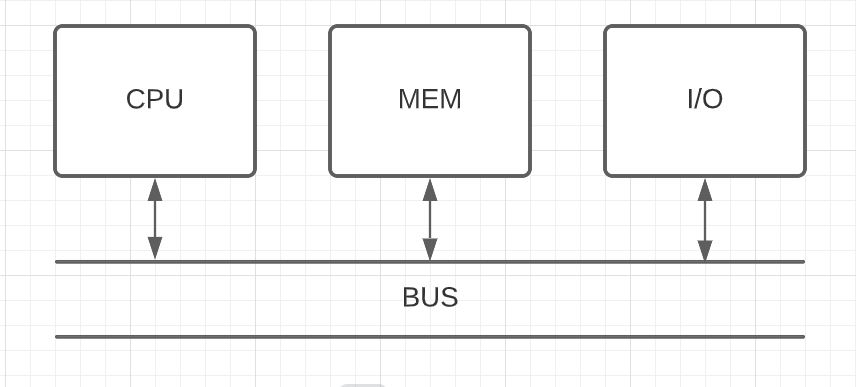
\includegraphics[width = 8cm]{images/modelloVonNeumann.JPG}
    \caption{Schematizzazione del modello Von Neumann}
    \label{modelloVonNeumann}
\end{figure}

\begin{itemize}
    \item La CPU (Central Processing Unit o processore) è formata da ALU (Unità Aritemtica Logica) che contiene tutti i circuiti per eseguire le operazioni aritmetico-logiche e la CU (o unità di controllo) che controlla l'esecuzione dei programmi;
    \item Nell'architettura dei calcolatori, si distinguono due tipi di memoria: la memoria centrale primaria, che lavora a più diretto contatto con il processore e la memoria secondaria o di massa;
    \item I dispositivi di Input/Output sono invece tutti quei dispositivi che non appartengono alla CPU o alla memoria;
    \item La CPU, la memoria e i dispositivi di Input/Output si scambiano i dati attraverso il Bus. Il Bus è l'insieme di linee su cui viaggiano i segnali elettrici formati da 0 e 1.
\end{itemize}
